% !TEX root = /Users/Gela/Desktop/Thesis_latex/thesis.tex
\section{Modeling}
Simscape software tool described in section Appendix A is used to do a physical model in order to achieve the characteristics of the membrane. The isolated system with pump, pipes, valves and water supply(tank) is implemented. Mass balance equations from section \ref{sec:soldiff} is used together with equations from \ref{sec:doweq}. The Temperature correction factor, $TCF$ is implemented with equation \ref{eq:TCF} to simulate the temperature dependency of the membrane. The osmotic pressure, $P_{osm}$ is implemented in the model by equation \ref{eq:feedOsmP}. The polariztion factor, $P_{f}$ that describes the polarization along the membrane surface is implemented with equation \ref{eq:polfac}. 
\\
\\
Dimensions on valves and pipes are implemented as the dimensions in the water device. Water quality, and temperature can be adjusted to simulate different conductivity and temperatures, to represent real values. The pump speed can be adjusted in the model to represent an actual value. Plots of characteristics of pressure, flow, salt concentration, temperature are received from the simulations, and can be seen in section \ref{sec:modres}

\section{Flowchart investigation}
\label{Flowchart}
Today, a system containing one pump is used. The pump is implemented at feed side of the membrane. The pump creates a pressure to overcome the osmotic pressure end create a flow from feed to permeate side. The system can be seen in \ref{fig:System11}. \\
\\
\begin{figure}[h]
    \centering
    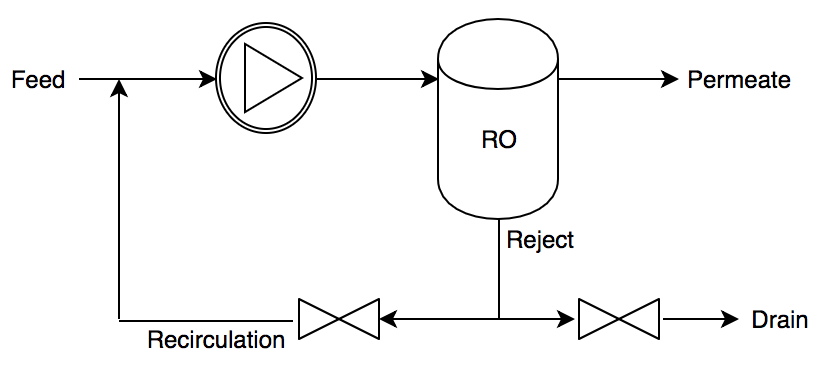
\includegraphics[width=0.5\textwidth]{Sys1}
    \caption{One pump system}
    \label{fig:System11}
\end{figure}
To obtain a system to investigate the membrane behaviour some different flowchart are considered. The current pump will be replaced by two pumps. Following requirements will be desirable when obtaining a updated model of the flowchart:
\begin{itemize}
\renewcommand\labelitemi{ }
\item Pressure drop over the membrane is high
\item Flow through membrane is high
\end{itemize}

\textbf{The model shall contribute with the following:}
\begin{itemize}
\renewcommand\labelitemi{ }
\item Permeate conductivity (minimised)
\item Fouling on the membrane (minimised)
\item Temperature dependencies 
\item Waste water going through drain (minimised)
\end{itemize}

\subsection{System 1}
Mainly two different systems containing two pumps were considered. The first system with one with pump on feed side and one pump on permeate side, as seen in Figure \ref{fig:FlowCInves1}. This setup contributes with the ability to create a net pressure over the membrane with a low, or even a under pressure on permeate side, whilst the feed pump creates a "high" pressure on feed side. Benefits with this implementation is the low energy consumption due to the ability to create negative pressure on permeate side. A high net driving pressure(pressure difference from feed to permeate side) can be achieved with rather low pressur on feed side. The withdrawal might be the implementation of the pump on permeate side. The water is used to feed dialysis machines and has high requirements on its purity. This sets high requirements on the pump, to not soil the purified water. 

\begin{figure}[h]
    \centering
    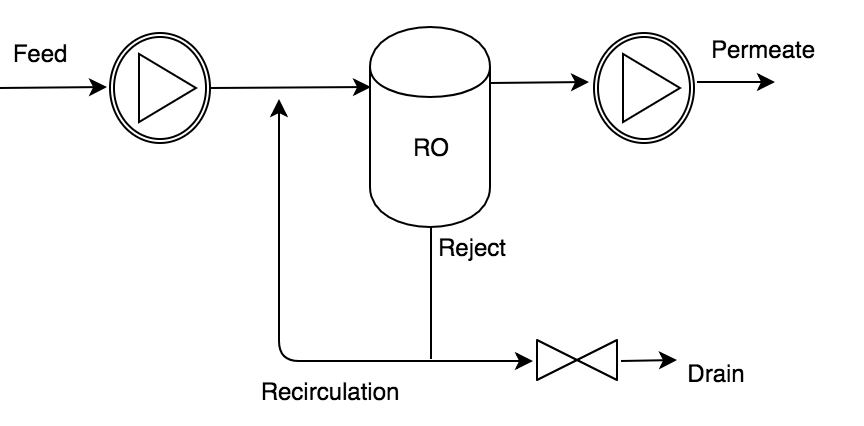
\includegraphics[width=0.4\textwidth]{FlowCInves1}
    \caption{System 1}
    \label{fig:FlowCInves1}
\end{figure}

\subsection{System 2}
The second system considered with one pump on feed side and one pump on reject side, in recirculation path, seen in Figure \ref{fig:Sys2}. The feed pump is used to create a high pressure on feed side and the pump in the recirculation path is used to control the flow in recirculation path. This contributes to control the recovery rate. Due to theory the membrane behaviour is dependent on feed and flow characteristics over the membrane, salt concentration and temperature. with this two pump solution the flow and pressure can be controlled independently and the membrane behaviour can be improved. The quality of the permeate water is ensured. \\
\\
\begin{figure}[h]
    \centering
    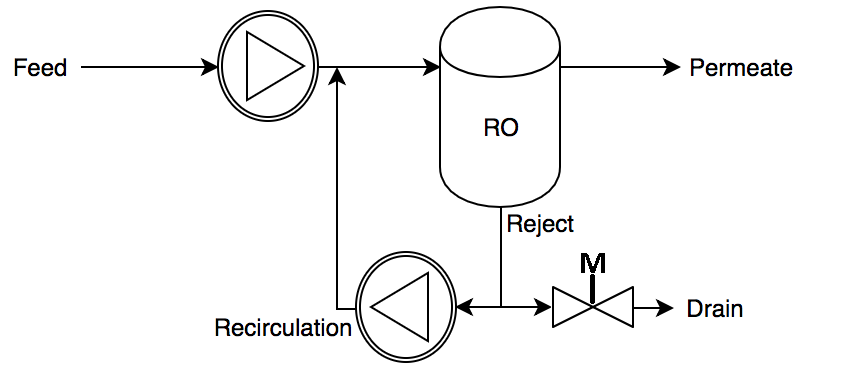
\includegraphics[width=0.4\textwidth]{Sys2}
    \caption{System 2}
    \label{fig:Sys2}
\end{figure}
\newpage

System 1 and System 2 contributes with the ability to control pressure and flow characteristics over the membrane. The big withdrawal with the implementation of a pump on permeate side is considered a high risk implementation and might put patients to high risks. System 1 is therefore precluded.

\section{Mapping}
In order to investigate the performance of the membrane pressure, flow, conductivity and temperature is  measured and logged. In the systems there are critical values of high pressure on feed side and reject side which makes it difficult to find measurement equipment that can handle both the high pressure and relatively low flows with no loss of pressure and required accuracy. \\
\\
Due to lack of instruments that could measure the flow under the high pressure some mapping of the flow from the pumps were done. The flow stream through the pumps were measured at different RPM and with different pressure resistance on the outlet. The flow is depending on the RPM with negligible difference depending on the applied outlet pressure from the pump. The mapped flow has an accuracy of $\pm$10\%.

\section{Implementation Test Rig}
\subsection{Current System}
In order to run all tests a physical rig was built. A first version to meet the specifications of the system used in the current water device were built according to Figure \ref{fig:MeasCurrSys}, with all the measurement sensors implemented. The rig contained, at the first stage: 1 pump with power supply, 1 RO-membrane, 3 needle valve, 1 drain valve, 1 water bath, three measurement sensors, pipes and couplings. The water bath is used to simulate different inlet water temperatures. The needle valves is used to adjust the pressure in the system to correspond with the real pressure characteristic in the water device. \\
\\
In order to log all signals and to run the system the Real-Time Target Machine described in Appendix A is connected with all significant signals. A GUI designed in Simulink to control the rig is connected to the rig. All control and feedback signals to and from the rig is handled in a built Simulink workspace where it is able to log and export all data to be able to analyse the system behaviour. All signals are filtered and displayed in real-time on a screen. \\
\\

\begin{figure}[h]
    \centering
    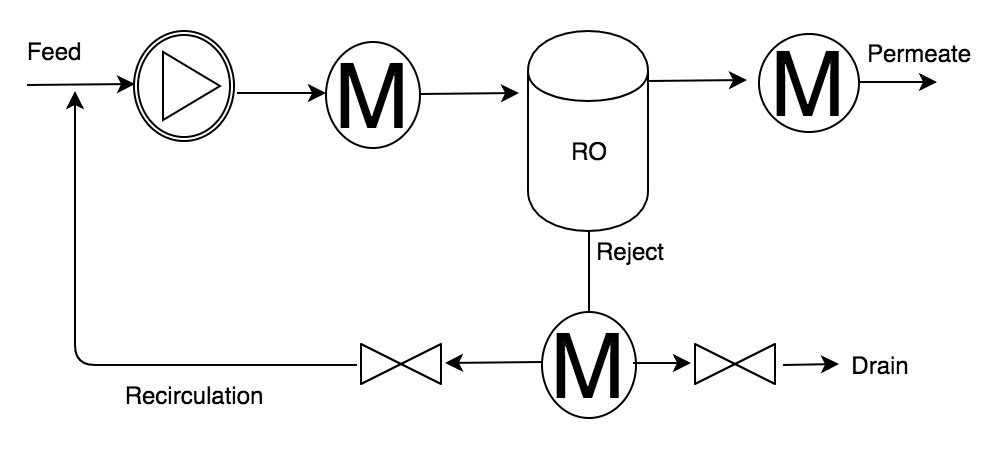
\includegraphics[width=0.4\textwidth]{MeasCurrSys}
    \caption{Current System, with measurement sensors}
    \label{fig:MeasCurrSys}
\end{figure}

\subsection{System 2  "Comparing system"}
The second system, System 2, were built by modifying the first rig, according to Figure \ref{fig:MeasSys2}. The second rig build contains: 2 pumps with power supply, 1 RO-membrane, 3 needle valve, 1 drain valve, 1 water bath, 1 flow meter, 3 measurement sensors, pipes and couplings. The water bath is used to simulate different inlet water temperatures. The needle valves is used to adjust the pressure in the system to correspond with the real pressure characteristic in the water device. The flow meter is used to measure the permeate flow from the membrane. \\
\\
The Simulink workspace, and the GUI was modified to be able to log all signal from the rig. All signals is displayed in real time as in the previous rig edition. Data is sampled and logged to be able to analyse the behaviour in the two pump system.  \\
\\
Different interfaces, as $i^{2}c$, Analog I/O, Digital inputs, PWM were used to implement the communication between the Real-Time Target Machine and measurement instruments. Circuits were built to transform voltage supply to required level for each component. All implementation of the communication and power supply can be seen in Figure \ref{fig:PressConn} - \ref{fig:PumpConn}. 

\begin{figure}[h]
    \centering
    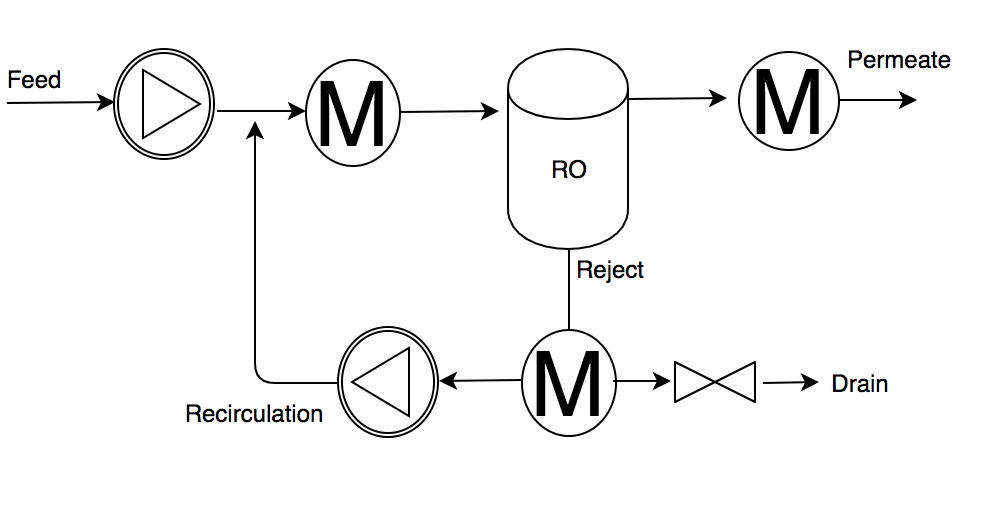
\includegraphics[width=0.4\textwidth]{MeasSys2}
    \caption{System 2, with measurement sensors}
    \label{fig:MeasSys2}
\end{figure}

\section{Test setup for membrane behaviour}
In order to compare results of the current system, furthermore called "Current System" and the updated system, System 2, some test will be done on the current setup. Reasonable values are investigated in order to meet requirements of the Water device. Corresponding points will be tested on the comparing system to evaluate any improvements on the membrane performance. The critical operational areas for the membrane is considered high temperatures (over 30 $^\circ$C) and high conductivity (over 2000 \SI{}{\micro\siemens}). The tests are performed in a range from 280-3000 \SI{}{\micro\siemens} and from 18-40 $^\circ$C. \\
\\
Points to be investigated can be seen in Table \ref{tab:testcases}. Same tests is performed on Current system and System 2 in order to analyse the difference in performance and membrane behaviour.\\
\begin{table}[h]
\begin{tabular}{|p{1.4cm}||p{2cm}|p{3.2cm}|p{1.8cm}|}
 \hline
 \textbf{Steady state }&Temperature&Feed Conductivity&Motor effect \\
 \hline
 1.1 & 18 $^\circ$C   & 280 \SI{}{\micro\siemens} & 60 \% \\
 1.2   &  18 $^\circ$C   & 500 \SI{}{\micro\siemens} & 60 \% \\
 1.3 &  18 $^\circ$C  &1000 \SI{}{\micro\siemens} & 60 \% \\
 1.4 &  18 $^\circ$C  &1000 \SI{}{\micro\siemens} & \textbf{80 \%} \\
 1.5 &18 $^\circ$C &2000 \SI{}{\micro\siemens}& 60 \%\\
 1.6 &18 $^\circ$C  &2000 \SI{}{\micro\siemens}& \textbf{80 \%}\\
 1.7   &18 $^\circ$C & 3000 \SI{}{\micro\siemens}&60 \% \\
 1.8   &18 $^\circ$C&3000 \SI{}{\micro\siemens}& \textbf{80 \%}\\
 \hline
 2.1 & 30 $^\circ$C & 280 \SI{}{\micro\siemens}&60 \%\\
 2.2 & 30 $^\circ$C &500 \SI{}{\micro\siemens}& 60 \%\\
 2.3 & 30 $^\circ$C&1000 \SI{}{\micro\siemens}& 60 \%\\
 2.4 & 30 $^\circ$C&1000 \SI{}{\micro\siemens}& \textbf{80 \%}\\
 2.5 & 30 $^\circ$C&2000 \SI{}{\micro\siemens}& 60 \%\\
 2.6 & 30 $^\circ$C&2000 \SI{}{\micro\siemens}& \textbf{80 \%}\\
 2.7 & 30 $^\circ$C& 3000 \SI{}{\micro\siemens}&60 \%\\
 2.8 & 30 $^\circ$C& 3000 \SI{}{\micro\siemens}&\textbf{80 \%}\\
 \hline 
 3.1 & 40 $^\circ$C& 280 \SI{}{\micro\siemens}& 60 \%\\
 3.2 & 40 $^\circ$C &500 \SI{}{\micro\siemens}& 60 \%\\
 3.3 & 40 $^\circ$C  & 1000 \SI{}{\micro\siemens}& 60 \%\\
 3.4 & 40 $^\circ$C  & 1000 \SI{}{\micro\siemens}& \textbf{80 \%}\\
 3.5 & 40 $^\circ$C&2000 \SI{}{\micro\siemens}& 60 \%\\
 3.6 & 40 $^\circ$C &2000 \SI{}{\micro\siemens}& \textbf{80 \%}\\
 3.7 & 40$^\circ$C &3000 \SI{}{\micro\siemens}& 60 \%\\
 3.8 & 40$^\circ$C &3000 \SI{}{\micro\siemens}& \textbf{80 \%}\\
\hline
\end{tabular}
\caption{Testcases}
    \label{tab:testcases} 
\end{table}


\newpage


\section{Design of control algorithms}

Investigating tests on System 2, Figure \ref{fig:Sys2}, were executed prior the design of the control algorithms to receive required reference signals to the pumps and drain valve. During the tests one parameter at a time changed while the others were kept constant. In test 1, seen in Figure \ref{fig:PreTestReg1} the pump in recycle path were the changing parameter and in Test 2, seen in Figure \ref{fig:PreTestReg3} the pressurising pump on inlet side were the changing parameter. 








